\subsection{Καταγραφή Χρόνων και Ανάλυση}

Όπως αναφέραμε και στο τέλος του προηγούμενου κεφαλαίου, το πείραμα υλοποιήθηκε σε δύο σκέλη και για κάθε ένα από αυτά, καταγράφηκε ο χρόνος που απαιτούταν μέχρι οι εθελοντές να ολοκληρώσουν τη διαδρομή τους, καθώς και το πλήθος των σφαλμάτων που πραγματοποιήσαν κατά τη διάρκεια αυτών. Οι χρόνοι αυτοί και τα σφάλματα έχουν αποτυπωθεί στον κατώθι πίνακα (\hyperref[tab:experimentTimeTable]{Πίνακας~\ref*{tab:experimentTimeTable}}).

%chktex-file 44

\begin{table}[!h]    
    \centering
    \caption{Αποτελέσματα χρονομετρήσεων των δύο σκελών του πειράματος}\label{tab:experimentTimeTable}
    \resizebox{\textwidth}{!}{%
    \begin{tabular}{c|c|c|c|c|c|c|c}
        \textbf{Εθελοντές} & \textbf{Σκέλος}   & \textbf{Τμήμα 1} & \textbf{Τμήμα 2} & \textbf{Τμήμα 3} & \textbf{Τμήμα 4} & \makecell{\textbf{Συνολικός} \\  \textbf{Χρόνος}} & \textbf{Σφάλματα} \\ \hline
            & (1) Μπαστούνι & 1:51.80 & 1:11.81 & 1:30.48 & 1.20:17 & 5:54.26 & 2 \\
        \rowcolor[HTML]{EFEFEF}
        \cellcolor[HTML]{FFFFFF} & (2) Εφαρμογή  & 3:29.77 & 2:19.55 & 2:48.95 & 3:11.17 & 11:49.44 & 2 \\
        \multirow{-3}{*}{Εθελοντής 1} & ---  & \cellcolor[HTML]{FD6864}+1:37.97 & \cellcolor[HTML]{FD6864}+1:07.74 & \cellcolor[HTML]{FD6864}+1:18.47 & \cellcolor[HTML]{FD6864}+1:51.00 & \cellcolor[HTML]{FD6864}+5:54.18 & \cellcolor[HTML]{9AFF99}0 \\ \hline
    
            & (2) Μπαστούνι & 00:53.73 & 00:42.71 & 00:59.75 & 1:10.66 & 3:46.85 & 3 \\
        \rowcolor[HTML]{EFEFEF}
        \cellcolor[HTML]{FFFFFF} & (1) Εφαρμογή  & 1:17.59 & 1:02.52 & 00:40.52 & 00:58.57 & 3:59.20 & 2 \\
        \multirow{-3}{*}{Εθελοντής 2} & ---  & \cellcolor[HTML]{FD6864}+00:23.86 & \cellcolor[HTML]{FD6864}+00:19.81 & \cellcolor[HTML]{9AFF99}-00:19.23 & \cellcolor[HTML]{9AFF99}-00:12.09 & \cellcolor[HTML]{FD6864}+00:12.62 & \cellcolor[HTML]{9AFF99}-1 \\ \hline

            & (1) Μπαστούνι & 1:22.74 & 00:51.50 & 1:16.73 & 1:41.63 & 5:12.60 & 3 \\
        \rowcolor[HTML]{EFEFEF}
        \cellcolor[HTML]{FFFFFF} & (2) Εφαρμογή  & 00:56.14 & 00:47.72 & 1:07.44 & 1:19.26 & 4:10.56 & 2 \\
        \multirow{-3}{*}{Εθελοντής 3} & ---  & \cellcolor[HTML]{9AFF99}-00:26.60 & \cellcolor[HTML]{9AFF99}-00:03.78 & \cellcolor[HTML]{9AFF99}-00:09.29 & \cellcolor[HTML]{9AFF99}-00:22.37 & \cellcolor[HTML]{9AFF99}-1:02.04 & \cellcolor[HTML]{9AFF99}-1 \\ \hline
    
            & (2) Μπαστούνι & 1:36.75 & 1:38.75 & 00:49.24 & 00:33.51 & 4:38.25 & 1 \\
        \rowcolor[HTML]{EFEFEF}
        \cellcolor[HTML]{FFFFFF} & (1) Εφαρμογή  & 3:12.21 & 1:43.52 & 2:31.27 & 00:50.25 & 8:19.60 & 9 \\
        \multirow{-3}{*}{Εθελοντής 4} & ---  & \cellcolor[HTML]{FD6864}+1:35.46 & \cellcolor[HTML]{FD6864}+00:04.77 & \cellcolor[HTML]{FD6864}+1:41.98 & \cellcolor[HTML]{FD6864}+00:16.74 & \cellcolor[HTML]{FD6864}+3:41.35 & \cellcolor[HTML]{FD6864}+8 \\ \hline
    
            & (1) Μπαστούνι & 1:39.21 & 00:58.62 & 00:22.51 & 00:48.58 & 3:48.92 & 7 \\
        \rowcolor[HTML]{EFEFEF}
        \cellcolor[HTML]{FFFFFF} & (2) Εφαρμογή  & 1:45.98 & 1:42.39 & 2:56.42 & 1:46.22 & 8:11.01 (*) & 9 \\
        \multirow{-3}{*}{Εθελοντής 5} & ---  & \cellcolor[HTML]{FD6864}+00:06.77 & \cellcolor[HTML]{FD6864}+00:43.77 & \cellcolor[HTML]{FD6864}+2:33.91 & \cellcolor[HTML]{FD6864}+00:57.64 & \cellcolor[HTML]{FD6864}+4:22.19 & \cellcolor[HTML]{FD6864}+2 \\ \hline
    
            & (2) Μπαστούνι & 1:12.96 & 00:30.83 & 00:47.95 & 00:30.06 & 3:01.80 & 3 \\
        \rowcolor[HTML]{EFEFEF}
        \cellcolor[HTML]{FFFFFF} & (1) Εφαρμογή  & 00:58.70 & 1:19.82 & 1:22.17 & 00:46.21 & 4:26.90 & 5 \\
        \multirow{-3}{*}{Εθελοντής 6} & ---  & \cellcolor[HTML]{9AFF99}-00:14.26 & \cellcolor[HTML]{FD6864}+00:48.99 & \cellcolor[HTML]{FD6864}+00:34.22 & \cellcolor[HTML]{FD6864}+00:16.15 & \cellcolor[HTML]{FD6864}+1:25.10 & \cellcolor[HTML]{FD6864}+2 \\ \hline
    
            & (1) Μπαστούνι & 00:25.97 & 00:17.66 & 00:38.77 & 00:50.15 & 2:12.55 & 1 \\
        \rowcolor[HTML]{EFEFEF}
        \cellcolor[HTML]{FFFFFF} & (2) Εφαρμογή  & 00:47.70 & 00:24.86 & 1:18.71 & 00:37.80 & 3:09.07 & 4 \\
        \multirow{-3}{*}{Εθελοντής 7} & ---  & \cellcolor[HTML]{FD6864}+00:21.73 & \cellcolor[HTML]{FD6864}+00:07.20 & \cellcolor[HTML]{FD6864}+00:39.44 & \cellcolor[HTML]{9AFF99}-00:12.35 & \cellcolor[HTML]{FD6864}+00:56.53 & \cellcolor[HTML]{FD6864}+3 \\ \hline
    
            & (2) Μπαστούνι & 1:01.52 & 00:36.82 & 00:47.83 & 00:39.70 & 3:05.87 & 2 \\
        \rowcolor[HTML]{EFEFEF}
        \cellcolor[HTML]{FFFFFF} & (1) Εφαρμογή  & 1:53.22 & 1:17.36 & 1:38.00 & 00:42.01 & 5:30.59 & 4 \\
        \multirow{-3}{*}{Εθελοντής 8} & ---  & \cellcolor[HTML]{FD6864}+00:51.30 & \cellcolor[HTML]{FD6864}+00:40.56 & \cellcolor[HTML]{FD6864}+00:50.17 & \cellcolor[HTML]{FD6864}+00:02.31 & \cellcolor[HTML]{FD6864}+2:24.72 & \cellcolor[HTML]{FD6864}+2 \\ \hline
    
            & (1) Μπαστούνι & 00:17.62 & 1:12.71 & 00:30.90 & 00:34.61 & 2:35.84 (*) & 1 \\
        \rowcolor[HTML]{EFEFEF}
        \cellcolor[HTML]{FFFFFF} & (2) Εφαρμογή  & 00:40.85 & 00:47.85 & 1:07.61 & 1:33.24 & 4:09.55 (*) & 3 \\
        \multirow{-3}{*}{Εθελοντής 9} & ---  & \cellcolor[HTML]{FD6864}+00:23.23 & \cellcolor[HTML]{9AFF99}-00:24.86 & \cellcolor[HTML]{FD6864}+00:36.71 & \cellcolor[HTML]{FD6864}+0:58.83 & \cellcolor[HTML]{FD6864}+1:33.71 & \cellcolor[HTML]{FD6864}+2 \\ \hline
    
            & (2) Μπαστούνι & 00:54.46 & 00:24.92 & 00:27.38 & 00:23.54 & 2:10.30 & 2 \\
        \rowcolor[HTML]{EFEFEF}
        \cellcolor[HTML]{FFFFFF} & (1) Εφαρμογή  & 1:54.47 & 00:51.47 & 1:18.27 & 00:28.25 & 4:32.46 & 3 \\
        \multirow{-3}{*}{Εθελοντής 10} & ---  & \cellcolor[HTML]{FD6864}+1:00.01 & \cellcolor[HTML]{FD6864}+00:26.55 & \cellcolor[HTML]{FD6864}+00:50.89 & \cellcolor[HTML]{FD6864}+00:04.71 & \cellcolor[HTML]{FD6864}+2:22.16 & \cellcolor[HTML]{FD6864}+1 \\ \hline
    \end{tabular}%
    }
\end{table}

Για κάθε εθελοντή, σημειώνουμε το χρόνο, ανά τμήματα της διαδρομής, καθώς και τον συνολικό, μέχρι να ολοκληρώσει το task του σε κάθε σκέλος του πειράματος και το πλήθος των σφαλμάτων στα οποιά υπέπεσε. Στη στήλη \textbf{Σκέλος}, δίπλα από κάθε συσκευή, που κάθε εθελοντής χρησιμοποίησε για να περιηγηθεί στον χώρο, καταγράφεται η σείρα με την οποία υλοποίησε τα δύο σκέλη του πειράματος. Στη τρίτη γραμμή κάθε εθελοντή, σημειώνεται οι διαφορές των χρόνων/σφαλμάτων των δύο προηγούμενων γραμμών της ίδια στήλης. Με κόκκινο χρωματίζεται το κελί, όπου η χρήση της συσκεύης HoloLens 2 αποδείκτηκε πιο χρονοβόρα από τη χρήση του μπαστουνιού ή οδήγησε σε περισσότερα σφάλματα, ενώ με πράσινο χρώμα σημειώνεται η αντίθετη περίπτωση. Τέλος, παρατήρούμε ότι ορισμένες διαδρομές των εθελοντών 5 και 9 έχουν σημειωθεί με ένα αστερίσκο (*). Ο λόγος είναι ότι οι συγκεκριμένοι εθελοντές, κατά το ένα ή και τα δύο σκέλη, περιηγήθηκαν στο χώρο κατά την αντίθετη φορά από τους υπόλοιπους. Ωστόσο, οι χρόνοι ανά τμήμα καταγράφηκαν έτσι ώστε να αναφέρονται στο ίδιο τμήμα.

Μπορούμε να παρατηρήσουμε ότι, για την πλειονότητα των εθελοντών, η χρήση της συσκευής HoloLens 2 οδήγησε σε αύξηση του χρόνου ολοκλήρωσης της προδιαγεγραμμένης διαδρομής. Εξαίρεση αποτελούν οι εθελοντές 2, 6, 7 και 9, οι οποίοι πραγματοποιήσαν ταχύτερους χρόνους με τη χρήση της εφαρμογής σε τμήματα της διαδρομής, καθώς και ο εθελοντής 3, ο οποίος παρουσίασε βελτιωμένη επίδοση στο σύνολο αυτής. Επίσης, τρεις στους δέκα εθελοντές είχαν μικρότερο αριθμό σφαλμάτων με τη χρήση της εφαρμογή σε σχέση με τη χρήση του μπαστουνιού. Ωστόπο, πρέπει να αντιληφθούμε ότι η προσέγγιση του πειράματος από τους εθελοντές παρουσιάζει πολλές διακυμάνσεις. Ειδικότερα, το εύρος του χρόνου ολοκλήρωσης της διαδρομής με το μπαστούνι είναι από $2:10.30$ έως $5:54.26$, ενώ με την εφαρμογή ξεκινά από $3:09.07$ έως και $11:49.44$. Επομένως, αρχικά, υπολογίσαμε τους μέσους χρόνους ολοκλήρωσης του task.

%chktex-file 44

\begin{table}[!h]
    \centering
    \caption{Μέσος χρόνο ολοκλήρωσης τμημάτων του πειράματος και μέσο πλήθος σφαλμάτων ανά σκέλος}\label{tab:experimentTimeTableMean}
    \resizebox{\textwidth}{!}{%
    \begin{tabular}{c|c|c|c|c|c|c}
        \textbf{Μέσος Χρόνος} & \textbf{Τμήμα 1} & \textbf{Τμήμα 2} & \textbf{Τμήμα 3} & \textbf{Τμήμα 4} & \makecell{\textbf{Συνολικός} \\ \textbf{Χρόνος}} & \textbf{Σφάλματα} \\ \hline
        Μπαστούνι & 01:07.68 & 00:50.63 & 00:49.15 & 00:51.26 & 03:38.72 & 2.5 \\ \hline
        Εφαρμογή & 01:50.29 & 01:13.71 & 01:40.94 & 01:13.30 & 05:49.84  & 4.3 \\ \hline
        --- & -00:42.61 & -00:23.08 & -00:51.81 & -00:22.04 & -02:11.12 & -1.8 \\ \hline
    \end{tabular}%
    }
\end{table}

\begin{table}[!h]
    \centering
    \caption{Μέση ποσοστιαία διαφορά χρόνων και ποσοστιαία διαφορά μέσων χρόνων ολοκλήρωσης τμημάτων του πειράματος}\label{tab:experimentTimeTablePercentageDiff}
    \resizebox{\textwidth}{!}{%
    \begin{tabular}{c|c|c|c|c|c}
            & \textbf{Τμήμα 1} & \textbf{Τμήμα 2} & \textbf{Τμήμα 3} & \textbf{Τμήμα 4} & \textbf{Συνολικός Χρόνος} \\ \hline
        \makecell{\textbf{Μέση Ποσοστιαία} \\ \textbf{Διαφορά Χρόνων}} & +68.25\% & +59.5\% & +151.73\% & +49.22\% & +61.64\% \\ \hline
        \makecell{\textbf{Ποσοστιαία Διαφορά} \\ \textbf{Μέσων Χρόνων}} & +62.96\% & +45.56\% & +105.34\% & +42.98\% & +59.94\% \\ \hline
    \end{tabular}%
    }
\end{table}

Με τη χρήση του μπαστουνιού, ο μέσος χρόνος ολοκλήρωσης της διαδρομής είναι $3:38.72$ με $2.5$ σφάλματα. Αντίθετα, με τη χρήση της εφαρμογής, οι εθελοντές ολοκλήρωναν τη διαδρομή με μέσο χρόνο τα $5:49.84$ και $4.3$ σφάλματα (\hyperref[tab:experimentTimeTableMean]{Πίνακας~\ref*{tab:experimentTimeTableMean}}). Δηλαδή παρατηρούμε αύξηση κατά δύο λεπτά περίπου στο μέσο χρόνο ολοκλήρωσης.

Επιπλέον υπολογίσαμε δύο ακόμη μεγέθη (\hyperref[tab:experimentTimeTablePercentageDiff]{Πίνακας~\ref*{tab:experimentTimeTablePercentageDiff}}). Αρχικά, υπολογίσαμε τη μέση ποσοστιαία διαφορά των χρόνων εθελοντών, το οποίο μας επιτρέπει να αντιληφθούμε σε ποια τμήματα παρουσιαζόταν η μεγαλύτερη διαφορά μεταξύ των χρόνων των δύο μεθόδων περιήγησης. Όπως παρατηρούμε, στο τμήμα 3 της διαδρομής, η διαφορά αυξάνεται ραγδαία, το οποίο δηλώνει δυσκολεύτηκαν ιδαίτερα με τη χρήση της εφαρμογής. Η αύξηση, όπως παρατηρήσαμε και κατά το πείραμα, οφείλεται στο γεγονός ότι στο συγκεκριμένο τμήμα, στη διαδρομή εμφανιζόταν ένα στένο πέρασμα, το οποίο δυσκολεύτηκαν να αντιληφθούν οι εθελοντές με την εφαρμογή. Στη συνέχεια, καταγράψαμε τη ποσοστιαία διαφορά των μέσων χρόνων, με το οποίο μπορούμε να αντιληφθούμε πόσο σημαντική ήταν η αύξηση του χρόνου στην περίπτωση της εφαρμογή. Στην πλεινότητα των τμημάτων, ο χρόνος χρήσης της εφαρμογής ήταν $1.5$ φορές μεγαλύτερη από αυτόν με τη χρήση του μπαστουνιού. Εξαίρεση και σε αυτή την περίπτωση αποτελεί το τμήμα 3, όπου, λόγω της ίδιας δυσκολίας, οι εθελοντές χρειάστηκαν τον διπλάσιο χρόνο. Η ποσοστιαία διαφορά των χρόνων ενός εθελοντή ή των μέσων χρόνων ενός τμήματος προέκυψε με βάση τον τύπο:
\[
    \text{ΠΔ\%} = \frac{t_{\text{Εφαρμογή}} - t_{\text{Μπαστούνι}}}{t_{\text{Μπαστούνι}}} \times 100\%
\]

Για μια πιο πλήρη παρουσίαση των ανωτέρων δεδομένων, θα πραγματοποιήσουμε στατιστική ανάλυση αυτών. Ειδικότερα, εφόσον διεξήχθη ένα within-subjects πείραμα, όπου καταγράφηκαν οι επιδόσεις των εθελοντών υπό δύο συνθήκες (χρήση μπαστουνιού και χρήση εφαρμογής), θα πραγματοποιήσουμε ένα paired-samples t test με ανέξαρτητη μεταβλητή τον τρόπο υποβοήθησης των χρηστών για την περιήγηση τους στο χώρο~\cite{lazar_2017_research}. Απαραίτητες προϋποθέσεις για να εφαρμόσουμε ένα paired-samples t test είναι:
\begin{itemize}
    \item Η εξαρτημένη μεταβλητή να έχει συνεχείς τιμές.
    \item Οι παρατηρήσεις μας να είναι ανεξάρτητες η μία από την άλλην.
    \item Δεν υπάρχουν ακραίες τιμές
    \item Οι τιμές της εξαρτημένης μεταβλητής είναι κανονικά κατανεμημένες
\end{itemize}

Αρχικά θα μελετήσουμε τα δείγματα συνολικού χρόνου ολοκλήρωσης της διαδρομής που έπρεπε να ακολουθήσουν οι εθελοντές. Οι δύο πρώτες προϋποθέσεις γνωρίζουμε ότι ισχύουν, οπότε πρέπει να ελέγξουμε τις τελευταίες δύο, ελέγχοντας τη διαφορά των χρόνων για τους εθελοντές. Η διαφορά ορίζεται ως:
\[
    t_{\text{Diff}} = t_{\text{Μπαστούνι}} - t_{\text{Εφαρμογή}}
\]

\begin{figure}[!h]
    \centering
    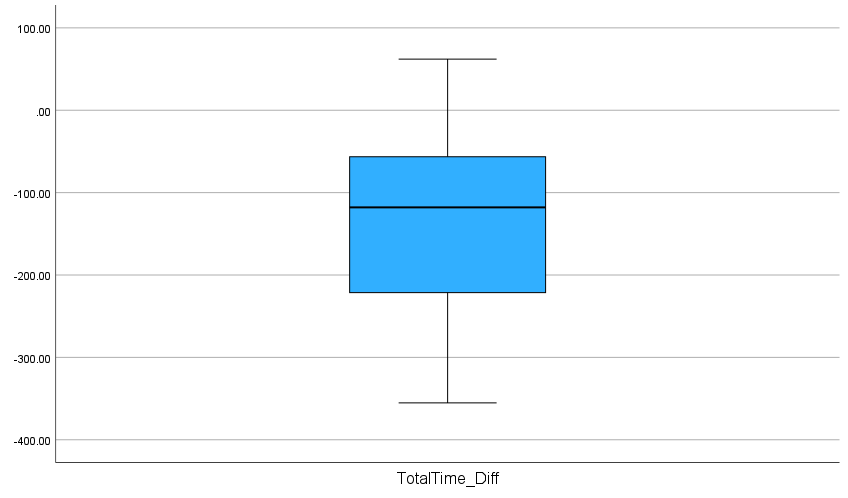
\includegraphics[width=0.8\linewidth]{./images/SA_Boxplot_TotalTimeDiff.png}
    \caption{Θηκόγραμμα της διαφοράς των συνολικών χρόνων}\label{fig:SABoxplotTTDiff}
\end{figure}

Με βάση το \hyperref[fig:SABoxplotTTDiff]{\schema~\ref*{fig:SABoxplotTTDiff}}, δεν παρατηρείται κάποια ακραία τιμή στο σύνολο των δειγμάτων μας.

\begin{figure}[!h]
    \centering
    \begin{subfigure}{0.8\textwidth}
        \centering
        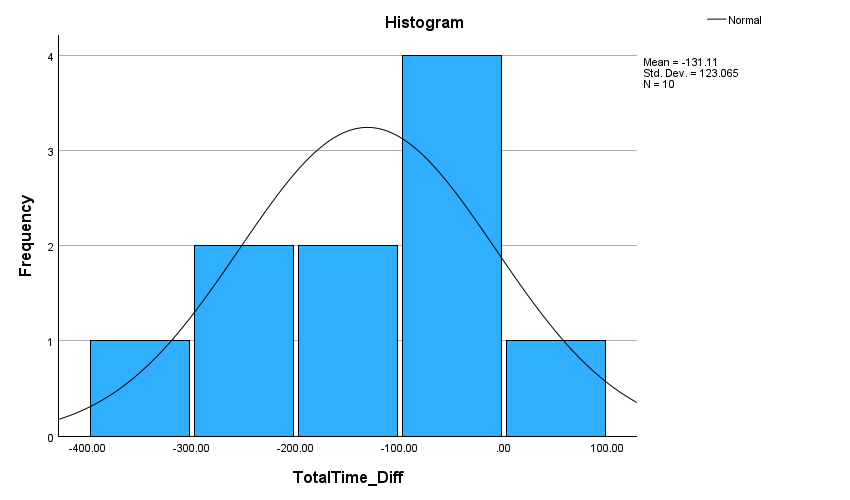
\includegraphics[width=1\linewidth]{./images/SA_Histogram_TotalTimeDiff.png}
        \caption{Ιστόγραμμα της διαφοράς των συνολικών χρόνων}
    \end{subfigure}%
    \\
    \begin{subfigure}{0.8\textwidth}
        \centering
        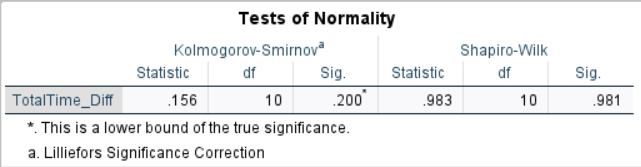
\includegraphics[width=1\linewidth]{images/SA_NormalityTest_TotalTimeDiff.png}
        \caption{Αποτελέσματα Normality Test}
    \end{subfigure}%
    \caption{Έλεγχος δειγμάτων για κανονική κατανομή στα δείγματα χρόνων ολοκλήρωσης}\label{fig:SANormalDistribution}
\end{figure}

Παρατηρώντας το \hyperref[fig:SANormalDistribution]{\schema~\ref*{fig:SANormalDistribution}}, διαπιστώνουμε ότι τα δεδομένα μας είναι κανονικά κατανεμημένα, λόγω της μορφής του ιστογράμματος, καθώς και ότι $p = 0.981 > 0.05$, που προκύπτει από το test Shapiro-Wilk~\cite{shapiro_1965_an}.

Επομένως, με βάση τα ανωτέρω, καλύπτουμε τις προϋποθέσεις για να πραγματοποιήσουμε ένα paired-samples t test. Αρχικά, εκφράζουμε τις υποθέσεις μας:
\begin{itemize}
    \item \textbf{$H_0$}: Η χρήση της συσκευής HoloLens 2 και της εφαρμογής δεν οδηγεί σε μικρότερο χρόνο ολοκλήρωσης της διαδρομής ($\mu_{\text{Μπαστούνι}} - \mu_{\text{Εφαρμογή}} \le 0$)
    \item \textbf{$H_{\text{a}}$}: Η χρήση της συσκευής HoloLens 2 και της εφαρμογής οδηγεί σε μικρότερο χρόνο ολοκλήρωσης της διαδρομής ($\mu_{\text{Μπαστούνι}} - \mu_{\text{Εφαρμογή}} > 0$)
\end{itemize}

Για να απορρίψουμε την μηδενική υπόθεση, πρέπει να είναι $t > t_{9,0.05}$, όπου $t_{9,0.05} = 1.833$ και για να θεωρηθούν τα αποτελέσματά μας στατιστικά σημαντικά, πρέπει $p < 0.05$.

Από τα αποτελέσματα (\hyperref[fig:SATTestTTDiff]{\schema~\ref*{fig:SATTestTTDiff}}) προκύπτει ότι το αποτέλεσμα ήταν στατιστικά σημαντικό, καθώς $p = 0.004 < 0.05$. Επομένως, παρατηρείται σημαντική διαφορά μεταξύ των χρόνων που καταγράφηκαν κάτω από τις δύο συνθήκες. Ωστόσο δεν μπορούμε να απορρίψουμε την μηδενική υπόθεση, καθώς ισχύει: $t = -3.369 < t_{9,0.05}$. Συμπεραίνουμε ότι η χρήση της εφαρμογής \textbf{αύξησε} τον συνολικό χρόνο ολοκλήρωσης της διαδρομής κατά $131.11 \pm 38.92$ δευτερόλεπτα.

\begin{figure}[!h]
    \centering
    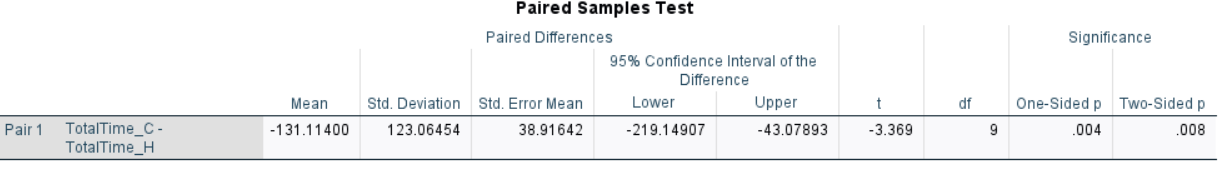
\includegraphics[width=1\linewidth]{./images/SA_TTestResult_TotalTimeDiff.png}
    \caption{Αποτελέσματα του paired-samples t test για τους χρόνους ολοκλήρωσης διαδρομής}\label{fig:SATTestTTDiff}
\end{figure}

Στη συνέχεια, εφαρμόζουμε μια παρόμοια διαδικασία και για τα δείγματα που αφορούν το σύνολο σφαλμάτων που πραγματοποίησαν οι εθελοντές κατά το πείραμα. Αρχικά ελέγχουμε αν τα δείγματα μας έχουν κάποια ακραία τιμή. Σε αυτήν την περίπτωση (\hyperref[fig:SABoxplotTEDiffWithOutliers]{\schema~\ref*{fig:SABoxplotTEDiffWithOutliers}}), παρατηρούμε ότι υπάρχουν ακραίες τιμές και ειδκότερα αυτές που αντλήσαμε από τον Εθελοντή 4. Οπότε, στη συνέχεια της ανάλυσης μας, θα αφαιρέσουμε το συγκεκριμένο δείγμα.

\begin{figure}[!h]
    \centering
    \begin{subfigure}{0.5\textwidth}
        \centering
        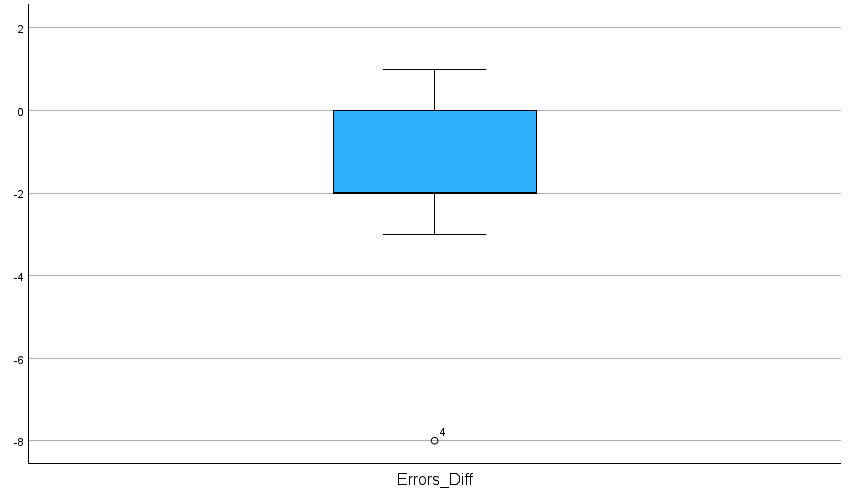
\includegraphics[width=0.9\linewidth]{images/SA_Boxplot_TotalErrorsDiff.png}
        \caption{Θηκόγραμμα με ακραία τιμή}\label{fig:SABoxplotTEDiffWithOutliers}
    \end{subfigure}%
    \begin{subfigure}{0.5\textwidth}
        \centering
        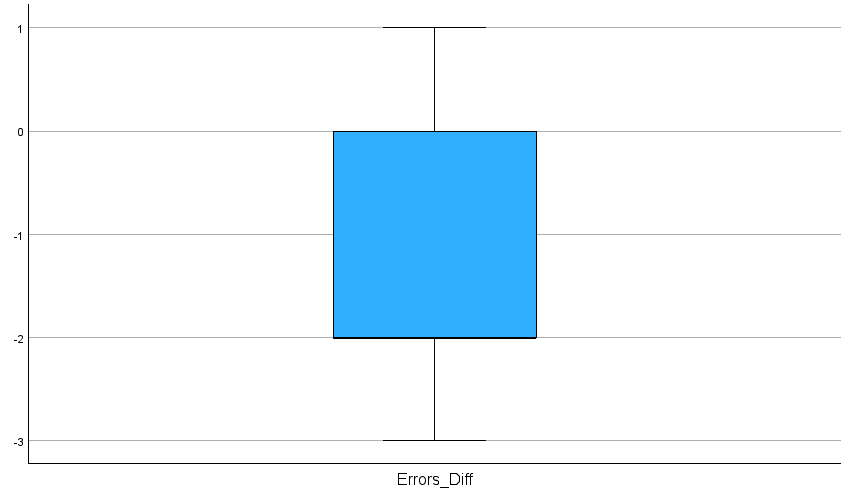
\includegraphics[width=0.9\linewidth]{images/SA_Boxplot_Without_Outliers_TotalErrorsDiff.png}
        \caption{Θηκόγραμμα χωρίς ακραία τιμή}\label{fig:SABoxplotTEDiffWithoutOutliers}
    \end{subfigure}%
    \caption{Θηκόγραμμα της διαφοράς του πλήθους σφαλμάτων}\label{fig:SABoxplotTEDiff}
\end{figure}

Αφού ελέγξαμε ότι τα δεδομένα παρουσιάζουν κανονική κατανομή (\hyperref[fig:SANormalDistributionTE]{\schema~\ref*{fig:SANormalDistributionTE}}), πραγματοποιούμε το paired-sampled t test με τις υποθέσεις:
\begin{itemize}
    \item \textbf{$H_0$}: Η χρήση της συσκευής HoloLens 2 και της εφαρμογής δεν οδηγεί σε μικρότερο αριθμό σφαλμάτων ($\mu_{\text{Μπαστούνι}} - \mu_{\text{Εφαρμογή}} \le 0$)
    \item \textbf{$H_{\text{a}}$}: Η χρήση της συσκευής HoloLens 2 και της εφαρμογής οδηγεί σε μικρότερο αριθμό σφαλμάτων ($\mu_{\text{Μπαστούνι}} - \mu_{\text{Εφαρμογή}} > 0$)
\end{itemize}

\begin{figure}[!hb]
    \centering
    \begin{subfigure}{0.8\textwidth}
        \centering
        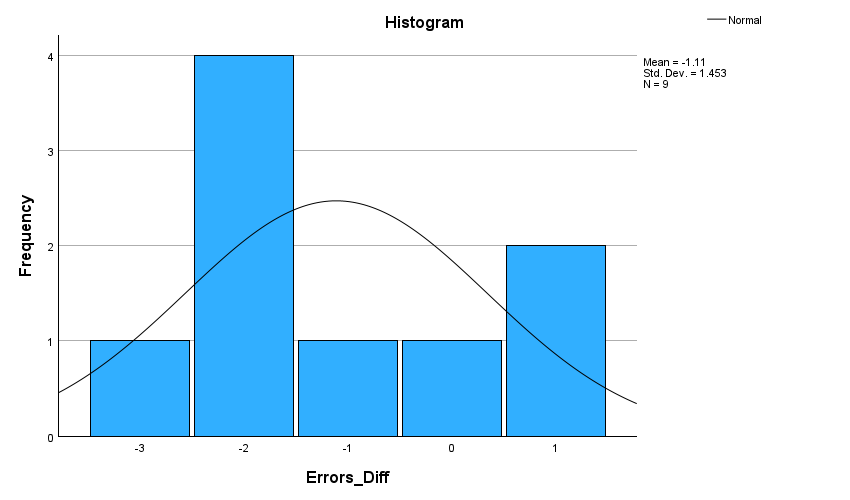
\includegraphics[width=1\linewidth]{./images/SA_Histogram_TotalErrorsDiff.png}
        \caption{Ιστόγραμμα της διαφοράς των σφαλμάτων}
    \end{subfigure}%
    \\
    \begin{subfigure}{0.8\textwidth}
        \centering
        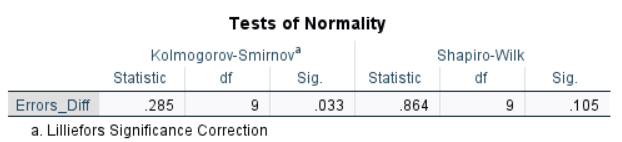
\includegraphics[width=1\linewidth]{images/SA_NormalityTest_TotalErrorsDiff.png}
        \caption{Αποτελέσματα Normality Test}
    \end{subfigure}%
    \caption{Έλεγχος δειγμάτων για κανονική κατανομή στα δείγματα σφαλμάτων}\label{fig:SANormalDistributionTE}
\end{figure}

Με βάση τα αποτελέσματα, όπως αυτά παρουσίαζονται στο \hyperref[fig:SATTestTEDiff]{\schema~\ref*{fig:SATTestTEDiff}}, πρόκειται για στατιστικά σημαντικά αποτελέσματα ($p = 0.025 < 0.05$), τα οποία, ωστόσο, δεν οδηγούν σε απόρριψη της μηδενικής υπόθεσης, καθώς ισχύει: $t = -2.294 < t_{8,0.05}$. Η μηδενική υπόθεση θα είχε απορριφθεί αν ίσχυε: $t > t_{8,0.05}$, όπου $t_{8,0.05} = 1.860$. Ειδικότερα, η χρήση της εφαρμογής οδηγεί σε $1.11 \pm 0.48$ \textbf{περισσότερα} σφάλματα από τη χρήση του μπαστουνιού.

\begin{figure}[!h]
    \centering
    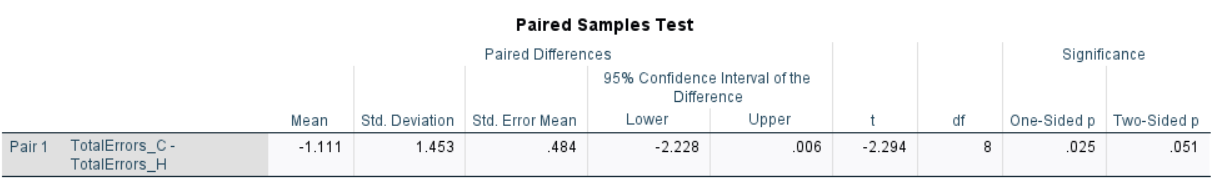
\includegraphics[width=1\linewidth]{./images/SA_TTestResult_TotalErrorsDiff.png}
    \caption{Αποτελέσματα του paired-samples t test για τους χρόνους ολοκλήρωσης διαδρομής}\label{fig:SATTestTEDiff}
\end{figure}

\subsection{Καταγραφή Απαντήσεων Ερωτηματολογίου και Παρατηρήσεις}

Μετά την ολοκλήρωση της πειραματικής διαδικασίας, οι εθελοντές έπρεπε να συμπληρώσουν ένα ερωτηματολόγιο. Το ερωτηματολόγιο αποτελούταν από μερικές εισαγωγικές ερωτήσεις, από τις οποίες προσπαθήσαμε να αντλήσουμε πληροφορίες σχετικά με προηγούμενες εμπειρίες των χρηστών με την τεχνολογία που μελετούσαμε. Στη συνέχεια συμπλήρωναν ένα ερωτηματολόγιο, το οποίο βασίστηκε στο ερωτηματολόγιο System Usability Scale (SUS), ενώ στο τέλος απάντησαν σε τρεις ερωτήσεις ανοικτού τύπου. Στο παρόν κεφάλαιο, θα αναλύσουμε τα δύο τελευταία τμήματα του ερωτηματολογίου.

Το SUS είναι ουσιαστικά μια κλίμακα Likert 5 σημείων~\cite{likert_1932_a} αποτελούμενη από δέκα προτάσεις. Οι εθελοντές επιλέγούν για κάθε πρόταση έναν αριθμό από το 1 έως το από 5 ανάλογα πόσο συμφωνούν ή διαφωνούν με την πρόταση αυτή. To SUS ερωτηματολόγιο δημιουργήθηκε με σκόπο να αποτέλεσει ένα σύντομο, εύκολο στη χρήση ερωτηματολόγιο, το οποίο περιγράφει την αντικειμενική χρηστικότητα ενός συστήματος ή μιας εφαρμογής. Οι προτάσεις έχουν διατυπωθεί με τέτοιο τρόπο, ώστε οι εθελοντές να επιλέγουν με σχετική ευκολία κάποιο άκρο της κλίμακας, έτσι ώστε να περιοριστούν ασαφείς απαντήσεις, δηλαδή απαντήσεις στη μέση της κλίμακας. Επίσης, οι θετικές και οι αρνητικές προτάσεις εναλλάσσονται έτσι ώστε ο εθελοντές να διατηρούν την προσοχή τους καθώς διαβάζουν τις προτάσεις~\cite{brooke_1995_sus}. Οι προτάσεις του ερωτηματολογίου παρατίθενται στο \hyperref[ch:appendixB]{Παράρτημα Β}, ενώ οι απαντήσεις των συμμετεχόντων ανά πρόταση στον \hyperref[tab:questionnaire]{Πίνακα~\ref*{tab:questionnaire}}. Συγκεκριμένα, στον πίνακα καταγράφουμε για κάθε πρόταση πόσοι εθελοντές επέλεξαν μία συγκεκριμένη βαθμίδα, ενώ στην τελευταία στήλη σημειώνουμε την μέση τιμή για τη συγκεκριμένη πρόταση.

%chktex-file 44

\begin{table}[!ht]
    \centering
    \resizebox{0.7\textwidth}{!}{%
    \begin{tabular}{c|c|c|c|c|c|c}
        \textbf{Προτάσεις} & \textbf{1} & \textbf{2} & \textbf{3} & \textbf{4} & \textbf{5} & \makecell{\textbf{Μέση} \\ \textbf{Τιμή}} \\ \hline
        Πρόταση 1 & 0 & 2 & 3 & 3 & 2 & 3.5 \\ \hline
        \rowcolor[HTML]{EFEFEF}
        Πρόταση 2 & 5 & 4 & 1 & 0 & 0 & 1.6 \\ \hline
        Πρόταση 3 & 0 & 0 & 3 & 3 & 4 & 4.1 \\ \hline
        \rowcolor[HTML]{EFEFEF}
        Πρόταση 4 & 5 & 2 & 2 & 1 & 0 & 1.9 \\ \hline
        Πρόταση 5 & 0 & 2 & 1 & 3 & 4 & 3.9 \\ \hline
        \rowcolor[HTML]{EFEFEF}
        Πρόταση 6 & 5 & 3 & 2 & 0 & 0 & 1.7 \\ \hline
        Πρόταση 7 & 0 & 0 & 1 & 3 & 6 & 4.5 \\ \hline
        \rowcolor[HTML]{EFEFEF}
        Πρόταση 8 & 7 & 3 & 0 & 0 & 0 & 1.3 \\ \hline
        Πρόταση 9 & 0 & 2 & 2 & 4 & 2 & 3.6 \\ \hline
        \rowcolor[HTML]{EFEFEF}
        Πρόταση 10 & 8 & 2 & 0 & 0 & 0 & 1.2 \\ \hline
    \end{tabular}%
    }
    \caption{Απαντήσεις στο ερωτηματολόγιο SUS}\label{tab:questionnaire}
\end{table}

Παράληλλα, στο \hyperref[fig:questionnaireSUSTotalScore]{\schema~\ref*{fig:questionnaireSUSTotalScore}} παρουσιάζουμε το συνολικό σκορ που καταγράφηκε για κάθε ερώτηση, δηλαδή το άθροισμα των βαθμών στην κλίμακα, που επέλεξαν οι εθελοντές για κάθε πρόταση. Όπως αναφέραμε προηγουμένως, οι θετικές και οι αρνητικές προτάσεις εναλλάσσονται. Επομένως, είναι σημαντικό οι ερωτήσεις με περιττό αύξοντα αριθμό να έχουν υψηλό σκορ, ενώ αυτές με ζυγό αύξοντα αριθμό να έχουν χαμηλό σκορ, ώστε το τελικό αποτέλεσμα να είναι θετικό. Αυτό γίνεται ξεκάθαρο και από τη σχέση με βάση την οποία υπολογίζεται το τελικό SUS Score:
\[
  \text{SUS Score} = 2.5 \times ( \sum_{n=1}^{5}(x_{2n - 1} - 1) + \sum_{n=1}^{5}(5 - x_{2n}))
\]

\begin{figure}[!ht]
    \centering
    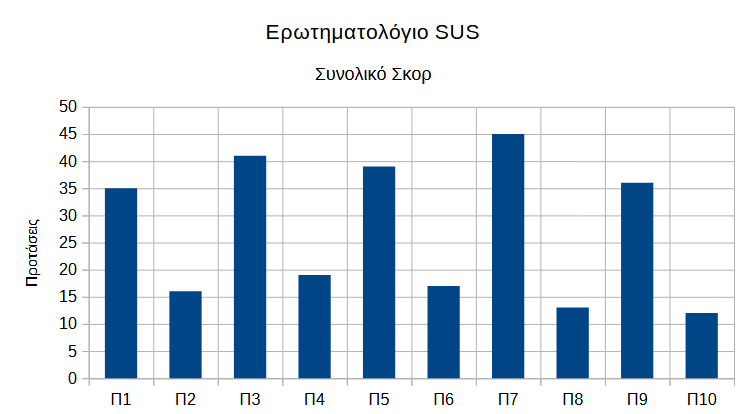
\includegraphics[width=1\textwidth]{./images/questionnaireSUSTotalScore.png}
    \caption{Συνολικό σκορ προτάσεων του ερωτηματολογίου SUS}\label{fig:questionnaireSUSTotalScore}
\end{figure}

Με βάση τις μέσες τιμές για κάθε πρόταση και την ανωτέρω σχέση, υπολογίζουμε ότι το τελικό SUS Score είναι $79.75 / 100$. Επομένως, παρά τις χαμηλές επιδόσεις της εφαρμογής όσον αφορά το χρόνο ολοκλήρωσης μιας διαδρομής και το πλήθος σφαλμάτων, οι εθελοντές αναγνωρίζουν τη χρηστικότητα της.

Οι λόγοι αυτής της αντίφασης γίνεται ξεκάθαροι με τη βοήθεια των ερωτήσεων ανοικτού τύπου, όπου οι εθελοντές εξηγούν τους λόγους για τους οποίους δυσκολεύτηκαν να ολοκληρώσουν το task σε χρόνο παρόμοιο ή ταχύτερο με αυτό του μπαστουνιού, καθώς και τι ήταν αυτό που ξεχώρισαν στην εφαρμογή. Οι ερωτήσεις ανοικτού τύπου απαντήθηκαν επί τον πλείστον με προφορικό τρόπο, ενώ ελάχιστοι ήταν που παρήχαν τις απαντήσεις τους γραπτά. Λόγω το πλήθος των απαντήσεων, στη συνέχεια, θα παραθέσουμε τα σημαντικότερα σημεία από αυτές, καθώς και ορισμένες από τις παρατηρήσεις μας.
\\[\baselineskip]
\begin{quote}
    \textbf{Ερώτηση 1}: Σας βοήθησε η εφαρμογή να αντιληφθείτε τη διάταξη του χώρου και να περιηγηθείτε σε αυτόν και με ποιον τρόπο;
\end{quote}

Η πλειονότητα των εθελοντών ανέφεραν ότι η εφαρμογή τους βοήθησε να αντιληφθούν τη διάταξη του χώρου, καθώς με μια απλή περιστρόφή, γνώριζαν που βρίσκονταν εμπόδια και σε ποια απόσταση, ενώ σε συνδυασμό με την αίσθηση του προσανατολισμού, γνώριζαν που βρίσκονταν στο χώρο. Ωστόσο υπήρχαν δύο εθελοντές, οι οποίοι ένιωσαν περισσότερη σιγουριά με το μπαστούνι και, όπως τονίζει ο ένας από αυτού, ο ήχος τον ανάγκαζε να επικεντρωθεί κυριώς στο τώρα και το εμπόδιο που αντιμετωπίζει, παρά να συγκεντρωθεί να σχηματίσει μια εικόνα του χώρου στο μυαλό του. Τέλος, ένας ακόμη εθελοντής τόνισε ότι το μπαστούνι τον βοήθησε να αντιληφθεί καλύτερα εμπόδια μικρά και αρκετά χαμηλά στο έδαφος.
\\[\baselineskip]
\begin{quote}
    \textbf{Ερώτηση 2}: Τι ήταν αυτό το οποίο σας δυσκόλεψε κάτα τη χρήση της εφαρμογής;
\end{quote}

Στο ερώτημα αυτό, όλοι οι εθελοντές ανέφεραν ελαττώματα σχετικά με τους προειδοποιητικούς ήχους. Ειδικότερα, εφτά στους δέκα εθελοντές σχολίασαν τη μίξη των προειδοποιητικών ήχων, το οποίο τους δυσκόλεψες να αντιληφθουν ποια είναι η σωστή απόσταση του εμποδίου. Το πρόβλημα είχε αναγνωριστεί πριν από πείραμα και αναφέρθηκε στο \hyperref[subsec:experimentSpecsForEvaluation]{Κεφάλαιο~\ref*{subsec:experimentSpecsForEvaluation}}. Οι υπόλοιποι ανέφεραν ότι το πλήθος των προειδοποιητικών ήχων, οι οποίοι διαφέρουν ως προς τη συχνότητα, τους δυσκόλεψε να διακρίνουν μεταξύ τους τα διαφορετικά επίπεδα προειδοποίησης. Τέλος, ένας εθελοντής σχολίασε ότι το χωρικός ήχος δεν ήταν ιδιαίτερα αισθητός και δεν τον βοήθησε να αντιληφθεί την κατεύθυνση του ήχου.
\\[\baselineskip]
\begin{quote}
    \textbf{Ερώτηση 3}: Ήταν κάτι το οποίο θεωρείτε ότι έλειπε από την εφαρμογή και θα σας διευκόλυνε την εμπειρία;
\end{quote}

Αρκετοί ήταν οι εθελοντές που ανέφεραν ότι θα προτιμούσαν λιγότερους και πιο ευδιάκριτους προειδοποιητικούς ήχους. Μερικοί πρόσθεσαν ότι σε κάποιο επίπεδο προειδοποίησης θα μπορούσε να αντικατασταθεί από άλλο τρόπο προειδοποίησης, όπως η απτική ανάδραση, οι φωτεινές σημάνσιες ή η εκφώνηση αναλυτικών οδηγιών ως προς την την ακριβή απόσταση των εμποδίων ή/και την κατεύθυνση που πρέπει να ακολουθήσει. Ορισμένες ακόμη ιδέες που προτάθηκαν ήταν η ενσωμάτωση αναγνώρισης εμποδίων, καθώς και η δυναμική αύξηση και μείωση του εύρους του cast, έτσι ώστε να εντοπίζονται ευκολότερα στενά περάσματα.

Όπως μπορούμε να αντιληφθούμε από τις ανωτέρω απαντήσεις, οι προειδοποιητικοί ήχοι ήταν αυτοί που αποτέλεσαν το κυριότερο μειονέκτημα της εφαρμογής και, όπως φαάνηκε, επηρέασαν σημαντικά τις επιδόσεις των εθελοντών σε σχέση με τη χρήση του μπαστουνιού, καθώς οι εθελοντές αναγκάζονταν συχνά να σταματήσουν και να περιμένουν μέχρις ότου γίνει ξεκάθαρο ποιος είναι ο σωστός προειδοποιητικός ήχος. Αιτία αυτού αποτελούν οι ασυνέπειες που δημιουργούνται στο mesh και η συχνή αλλαγή αυτού σε κάθε interval. Λύση σε αυτό θα μπορούσε να αποτελέσει η αντικατάσταση του Boxcast, το οποίο είναι ευαίσθητο στις ασυνέπειες αυτές, με collision detection, δηλαδή η δημιουργία ζωνών γύρω από το χρήστη και ηα αγνώριση συγκρούσεων του mesh εμποδίων με τις ζώνες αυτές. Ώστοσο, πέρα αυτού του προβλήματος, οι εθελοντές χαρακτήρισαν τη συσκεύη ιδιαίτερα άνετη και τη χρήση της εφαρμογής αρκετά απλή και κατανοητή και ιδιαίτερα χρηστική στο σύνολό της. Επίσης, με βάση τις απαντήσεις τους στο τελευταίο ερώτημα, φαίνεται ότι γίνεται ιδιαίτερα αντιληπτό η δυνατότητα συνεχής βελτίωσης της εφαρμογής και η ενσωμάτωση πολλών νέων δυνατοτήτων που εκμεταλλεύονται πληθώρα άλλων τεχνολογιών και αισθήσεων, κάτι το οποίο δύσκολα υλοποιείται σε ένα μπαστούνι.